\begin{figure*}[t]
  \centering
  \setlength{\tabcolsep}{1pt}
  \begin{tabular}{@{}c@{\hspace{2pt}}ccccc@{}}
    \rotatebox{90}{\makebox[0.247\linewidth][c]{\footnotesize Apple}} &
      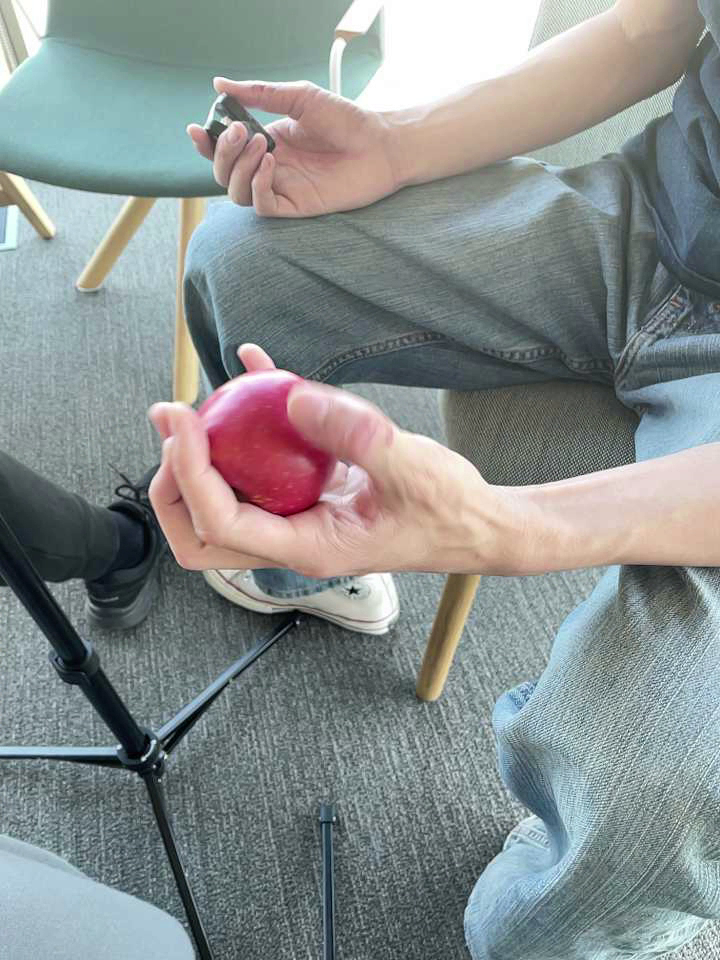
\includegraphics[width=0.185\linewidth]{img/comparison/apple_gt.png} &
      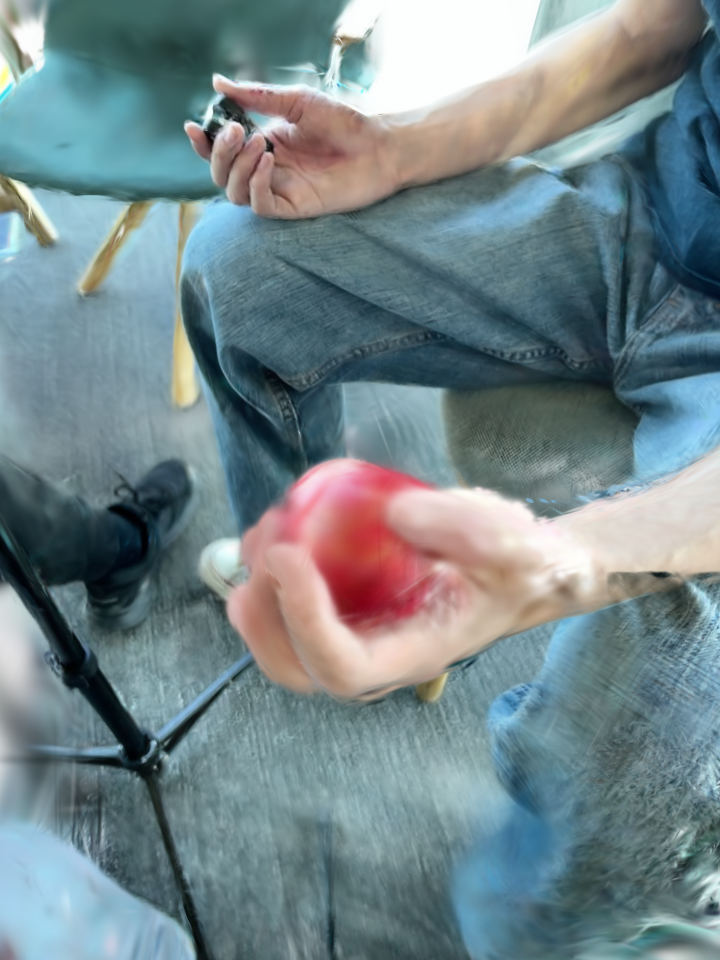
\includegraphics[width=0.185\linewidth]{img/comparison/apple_ours.png} &
      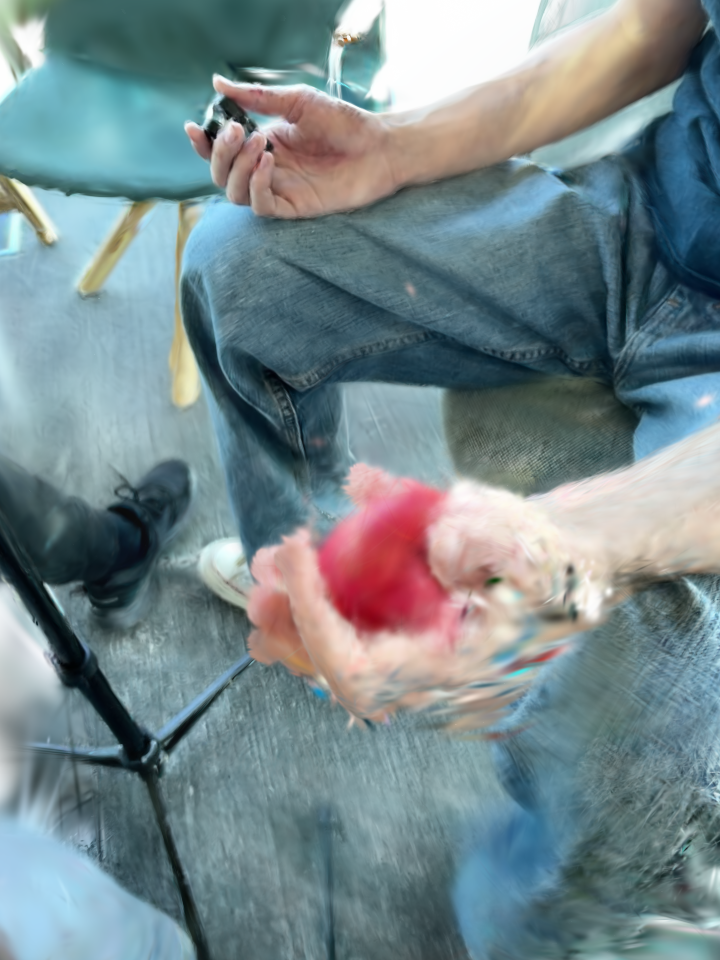
\includegraphics[width=0.185\linewidth]{img/comparison/apple_som.png} &
      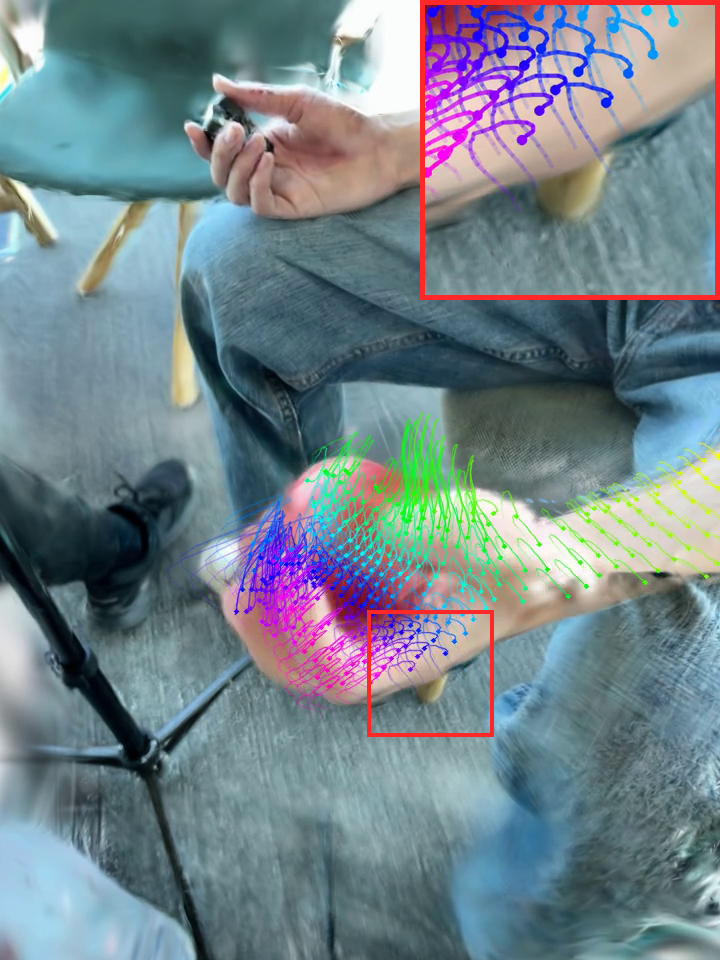
\includegraphics[width=0.185\linewidth]{img/comparison/apple_ours_tracks.png} &
      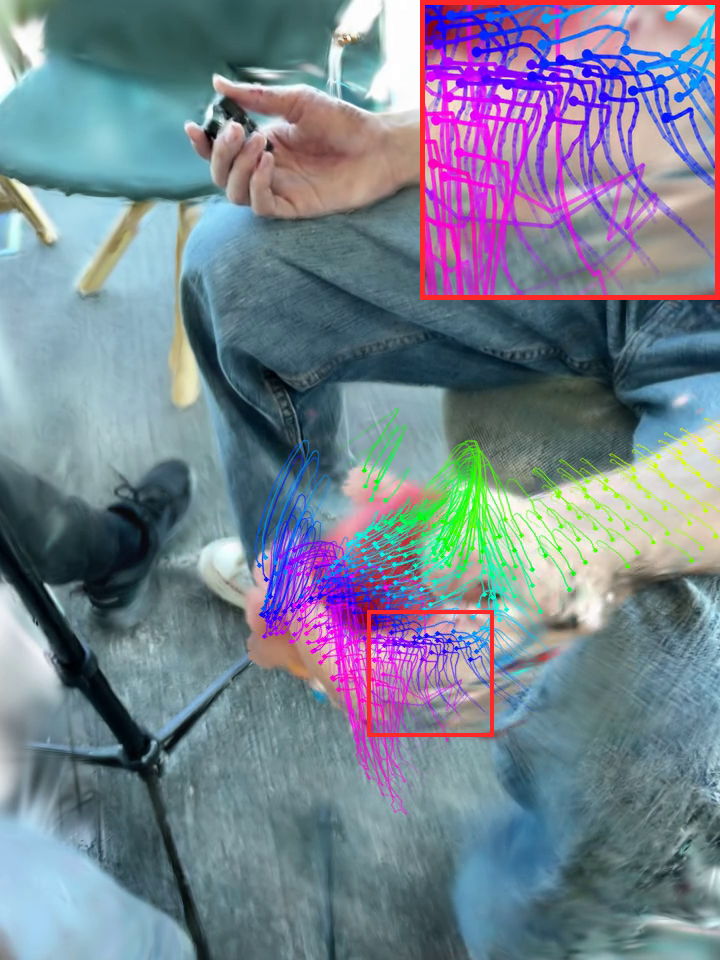
\includegraphics[width=0.185\linewidth]{img/comparison/apple_som_tracks.png} \\
    \rotatebox{90}{\makebox[0.247\linewidth][c]{\footnotesize Paper Windmill}} &
      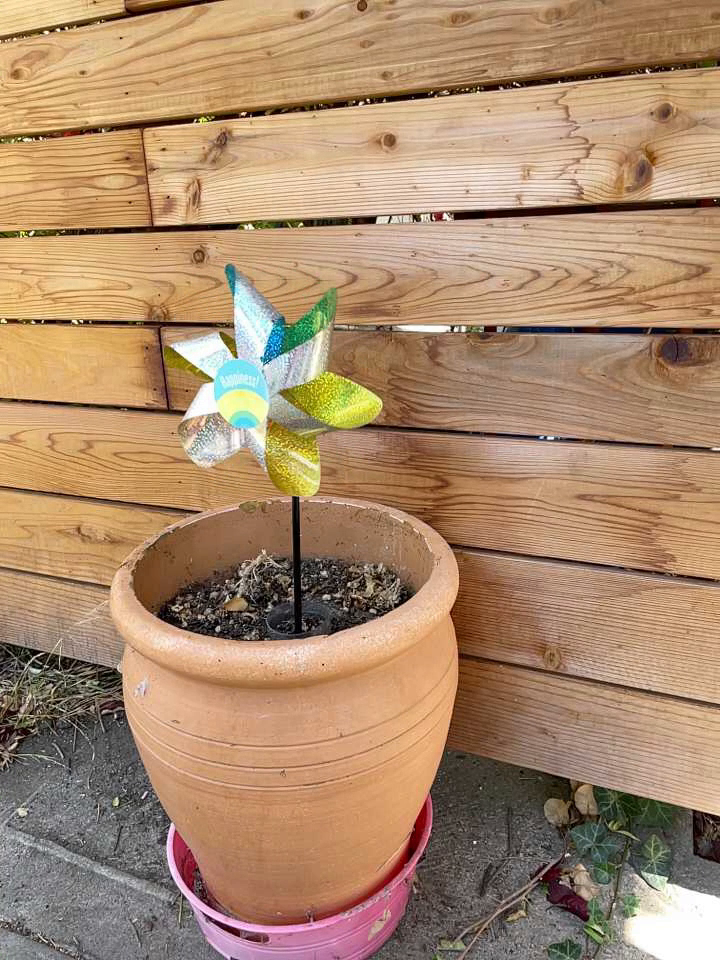
\includegraphics[width=0.185\linewidth]{img/comparison/windmill_gt.png} &
      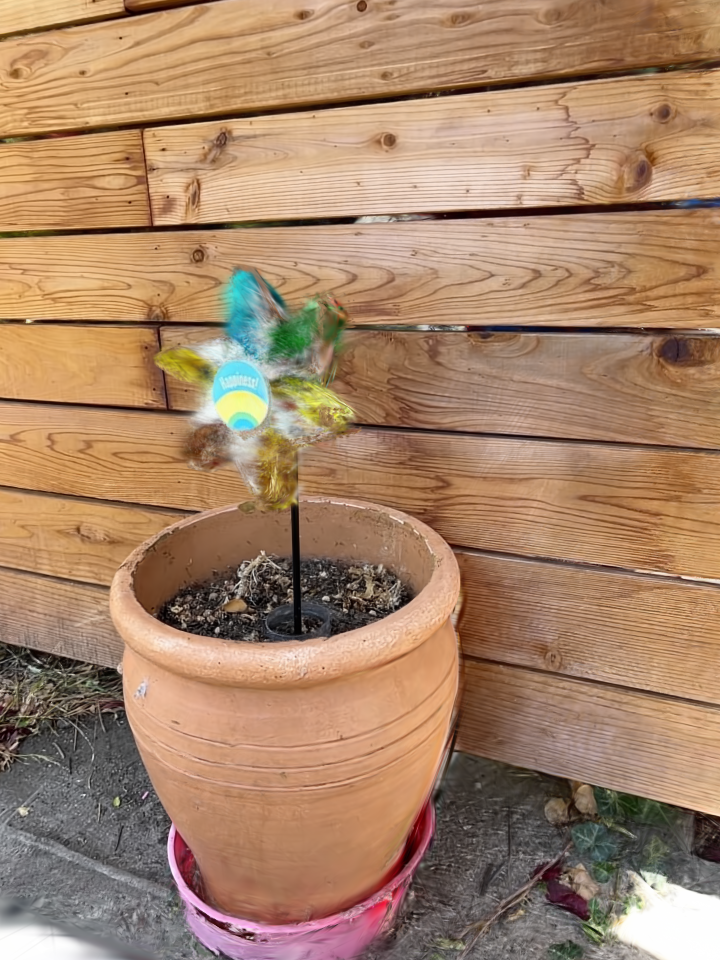
\includegraphics[width=0.185\linewidth]{img/comparison/windmill_ours.png} &
      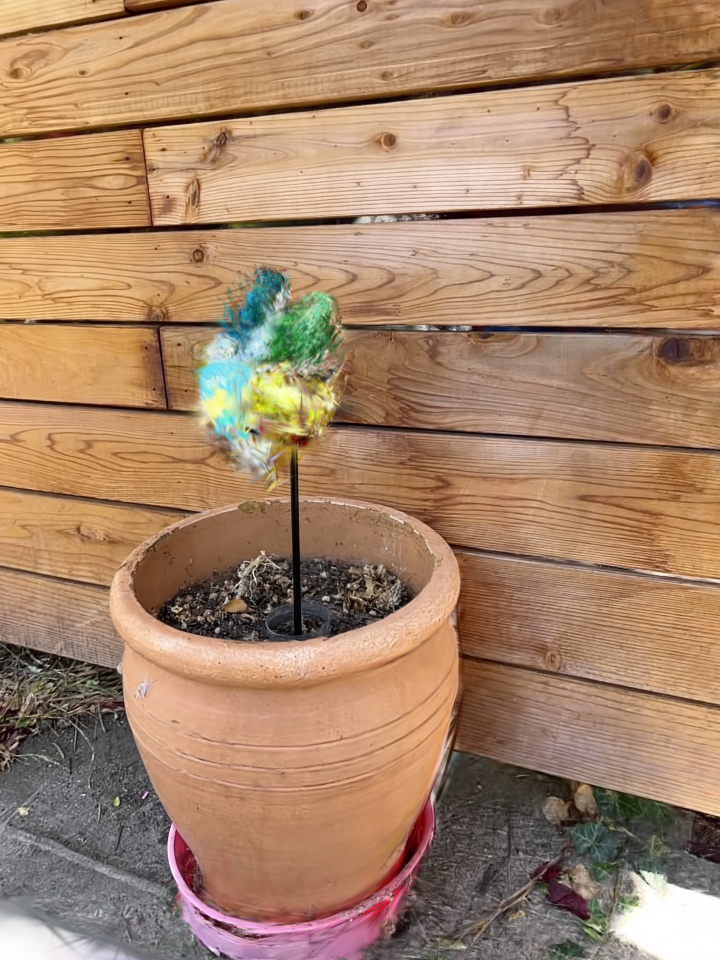
\includegraphics[width=0.185\linewidth]{img/comparison/windmill_som.png} &
      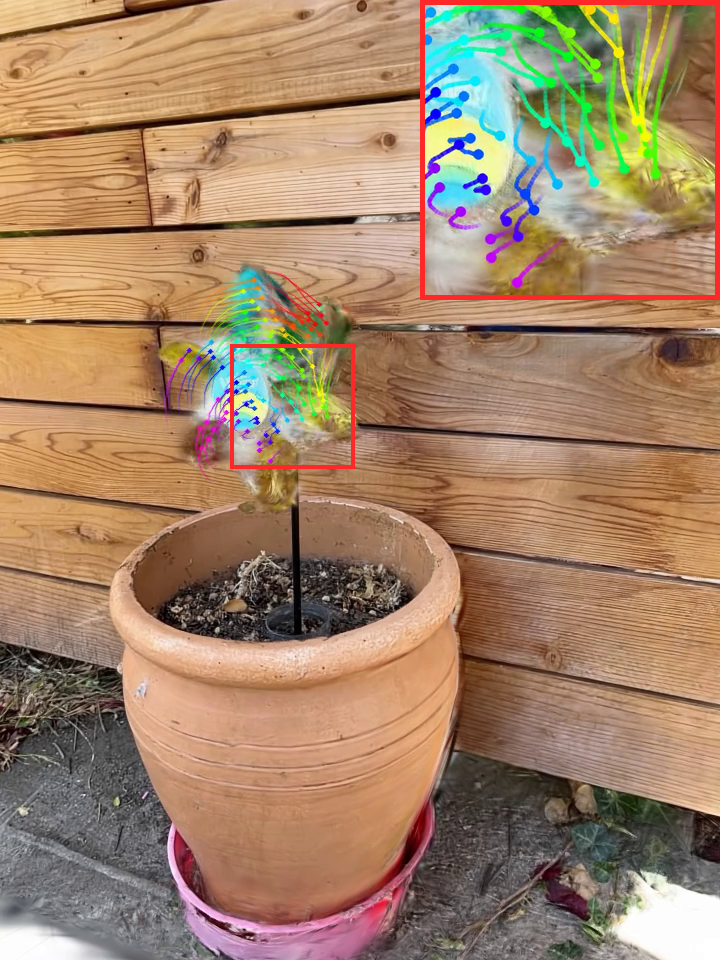
\includegraphics[width=0.185\linewidth]{img/comparison/windmill_ours_tracks.png} &
      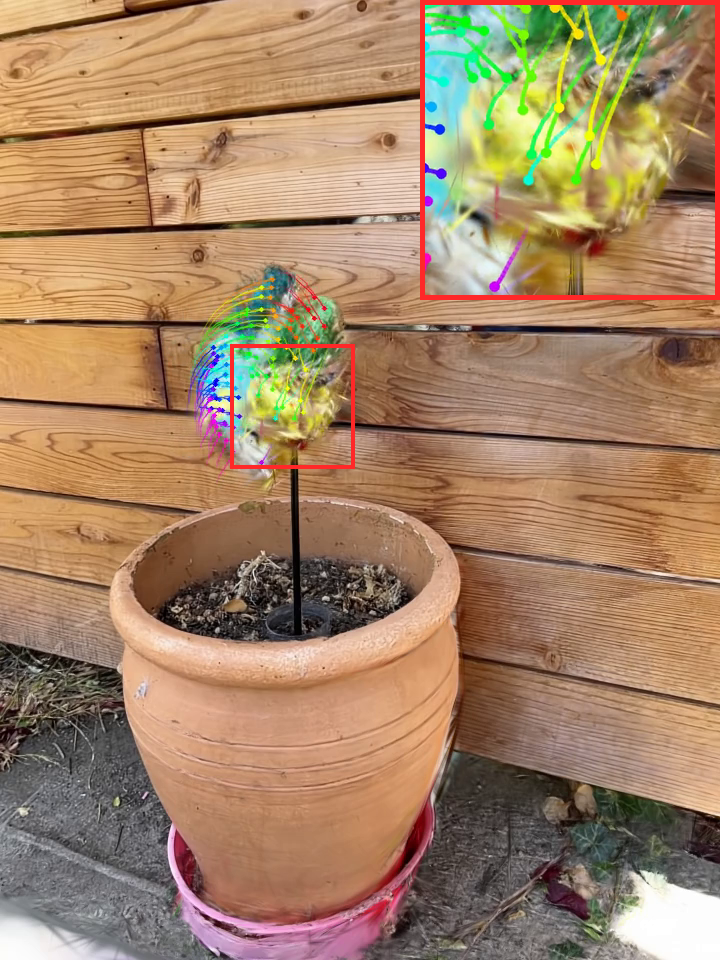
\includegraphics[width=0.185\linewidth]{img/comparison/windmill_som_tracks.png} \\
    
     & \makebox[0.185\linewidth][c]{\footnotesize GT (Test View)} &
       \makebox[0.185\linewidth][c]{\footnotesize Ours} &
       \makebox[0.185\linewidth][c]{\footnotesize SoM} &
       \makebox[0.185\linewidth][c]{\footnotesize Ours (Tracks)} &
       \makebox[0.185\linewidth][c]{\footnotesize SoM (Tracks)} \\
  \end{tabular}
 \caption{\lulu{Replace with updated visualizations + all the baselines}Our method retains regularization toward the main motion modes, while SoM overfits and degrades on the test view.}
  \label{fig:qualitative-comparison}
\end{figure*}
